\documentclass{beamer}
\usepackage{graphicx}

\usepackage{subfigure}

\usepackage{amsmath}
\usepackage{amssymb}

\usepackage{ulem}

\usepackage{url}

\usepackage{tikz}
\usetikzlibrary{calc,positioning,graphs,shapes,quotes,arrows}
\usepackage{ctex}
\usepackage{pgfplots}
\pgfplotsset{width=5cm,compat=1.9}

\usepackage{hyperref}
\hypersetup{hidelinks,
      colorlinks=true,
      allcolors=blue,
      pdfstartview=Fit,
      breaklinks=true}

\usepackage[backend=bibtex,sorting=none]{biblatex}
\addbibresource{Finalhw.bib}
\setbeamerfont{footnote}{size=\tiny}

\setlength{\parindent}{2em}
\usetheme{AnnArbor}
\usecolortheme{beaver}
\usefonttheme{default}
\setbeamertemplate{bibliography item}[text]

\title{一维非线性方程求根算法}

\author{赵天健 \\ 信息与计算科学\quad 3210101830}

\begin{document}
\begin{frame}
\titlepage
\end{frame}


\begin{frame}
\frametitle{引言}
很久以来, 解方程都是数学家们非常关注的问题. 而解方程最基本的就是解一元方程的问题. 不过, 非线性的一元方程求解并不容易, 就算对于多项式来说也是如此. 根据Abel-Ruffini定理, 对于多项式方程$p(x) = 0$来说, 若$\deg{p} \ge 5$, 那么其没有求根公式, 而一些非多项式方程的解析解就更加难求了. 但是, 很多时候我们仍然希望在某个区间$[l, r]$内找到方程$f(x) = 0$的解, 哪怕是数值上的近似解. 为了解决这个问题, 许多迭代算法应运而生.
\end{frame}


\begin{frame}
\frametitle{一些求根算法的介绍}
\end{frame}


\begin{frame}
\frametitle{二分法}
设$f(x)$是连续函数, 现有区间$[a, b]$, 且$f(a)f(b) < 0$, 那么取区间中点$c = \frac{a+b}{2}$, 则$[a, c], [b, c]$必有至少一个区间存在$f(x)$的根. 而由于连续函数的介值定理, 则函数值与$f(c)$符号相异的端点与$c$构成的区间内必然存在根.
\end{frame}

\begin{frame}
\frametitle{算法流程}
\begin{figure}[htb]
\centering
\begin{tikzpicture}[node distance=5pt, hv path/.style = {to path={-| (\tikztotarget) \tikztonodes}}]
\node[draw, rounded corners]						 (sstart)   {Start};
\node[draw, rounded corners, below=of sstart]		 (start)    {给定$f$和区间$[a, b]$};
\node[draw, diamond, aspect=2, below=of start]		 (choice 1) {$b - a < eps$};
\node[draw, below=of choice 1]                       (step 1)   {计算$[a, b]$中点$c$};
\node[draw, below=of step 1]                         (step 2)   {计算$f(c)$};
\node[draw, diamond, aspect=2, below=of step 2]      (choice 2) {$f(a)f(c) < 0$};
\node[draw, rounded corners, right=20pt of choice 1] (end)      {End};
\coordinate[right=10pt of end] 						 (px);
\coordinate[left=30pt of choice 1]					 (py);

\graph{
	(start) -> (choice 1) ->["No"left] (step 1) -> (step 2) -> (choice 2);
	(choice 1) -> ["Yes"](end);
};
\draw[->] (sstart) -- (start);
\draw[rounded corners] (choice 2) -- node[above, near start] {Yes} (choice 2-|px) -> (px);
\draw[->, rounded corners] (px) -- node[above, very near end] {$[a,c]$} (px|-start) -> (start);
\draw[rounded corners] (choice 2) -- node[above, near start] {No} (choice 2-|py) -> (py);
\draw[->, rounded corners] (py) -- node[above, very near end] {$[c,b]$} (py|-start) -> (start);
\end{tikzpicture}
\caption{二分法流程图}
\label{fig:bisection}
\end{figure}
\end{frame}


\begin{frame}
\frametitle{Newton法}
\begin{figure}[!ht]
	\centering
	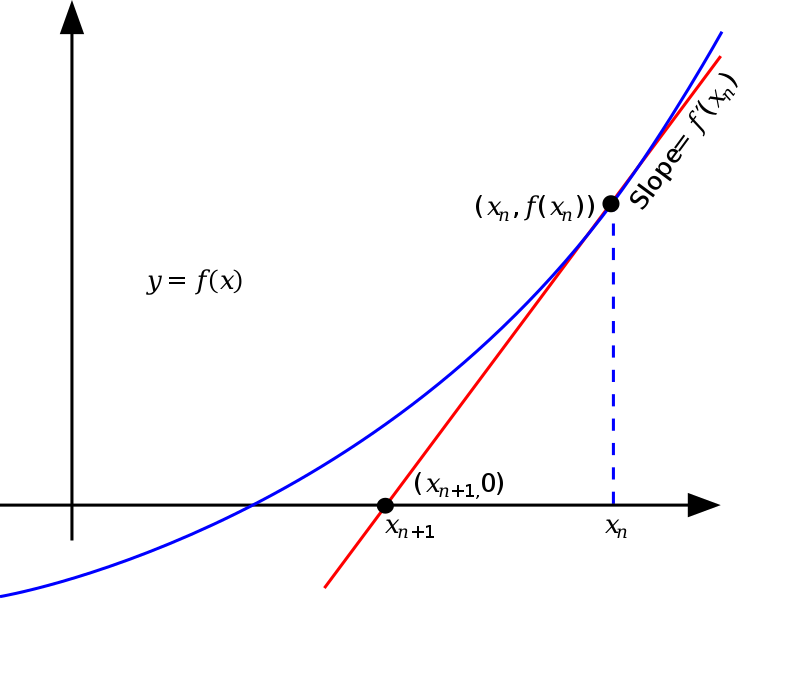
\includegraphics[width=3in]{../img/example.svg.png}
	\caption{$x_{n+1}$比$x_n$更好}
	\label{fig:wiki}
\end{figure}
\end{frame}

\begin{frame}
\frametitle{算法流程}
\begin{figure}[htb]
\centering
\begin{tikzpicture}[node distance=10pt, hv path/.style = {to path={-| (\tikztotarget) \tikztonodes}}]
\node[draw, rounded corners]						 (sstart)   {Start};
\node[draw, rounded corners, below=of sstart]		 (start)	{给定$f, f'$和$x_0$};
\node[draw, below=of start]							 (step 1)	{根据公式求出$x_1$};
\node[draw, diamond, aspect=2, below=of step 1]		 (choice 1) {$|x_1 - x_0| < eps$};
\node[draw, rounded corners, below=of choice 1]		 (end)		{end};
\coordinate[right=30pt of step 1]					 (px);

\graph{
	(sstart) -> (start) -> (step 1) -> (choice 1) -> ["Yes"left] (end);
};
\draw[rounded corners] (choice 1) -- node[above, near start] {No} (choice 1-|px) -> (px);
\draw[->, rounded corners] (px) -- node[above, very near end] {$x_1$} (px|-start) -> (start);

\end{tikzpicture}
\caption{Newton法流程图}
\label{fig:newton}
\end{figure}
\end{frame}

\begin{frame}
\frametitle{收敛速度比较}
\end{frame}

\begin{frame}
\frametitle{$f(x) = e^{2x}-2$}
\begin{figure}[htb]
\centering
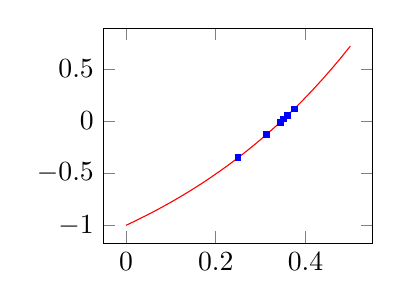
\begin{tikzpicture}
\begin{axis}
\addplot[domain=0:0.5, color=red]{exp(2 * x) - 2};
\addplot[only marks, mark=square*, color=blue, mark size=1pt]
coordinates{(0.25, -0.351278)(0.375, 0.117000)(0.3125, -0.131754)(0.34375, -0.011262)(0.359375, 0.051866)(0.351563, 0.020057)};
\end{axis}
\end{tikzpicture}
\caption{二分法}
\label{fig:bis_exp}
\end{figure}
\par 二分法迭代19次后达到目标精度.
\end{frame}

\begin{frame}
\frametitle{Newton法}
\begin{figure}[htb]
\centering
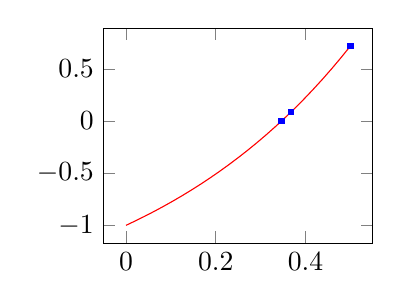
\begin{tikzpicture}
\begin{axis}
\addplot[domain=0:0.5, color=red]{exp(2 * x) - 2};
\addplot[only marks, mark=square*, color=blue, mark size=1pt]
coordinates{(0.5, 0.718282)(0.367879, 0.087063)(0.347021, 0.001790)(0.346573, 0)};
\end{axis}
\end{tikzpicture}
\caption{Newton法}
\label{fig:new_exp}
\end{figure}
\par 牛顿法迭代5次后即达到目标精度, 显著优于二分法.
\end{frame}

\begin{frame}
\frametitle{$f(x) = 8x^5 + x^4 + 9x^2 + 7x + 5$}
\begin{figure}[htb]
\centering
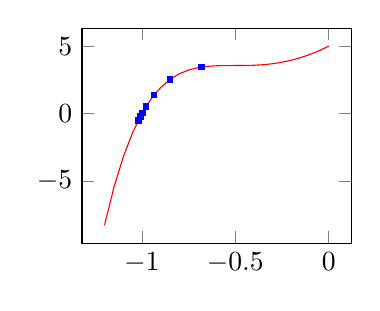
\begin{tikzpicture}
\begin{axis}
\addplot[domain=-1.2:0, color=red]{8*x^5 + x^4 + 9*x^2 + 7*x + 5};
\addplot[only marks, mark=square*, color=blue, mark size=1pt]
coordinates{(-0.679571, 3.453147)(-1.019356, -0.508801)(-0.849463, 2.530289)(-0.934409, 1.380867)(-0.976883, 0.544117)(-0.998119, 0.046796)(-1.008737, -0.223437)};
\end{axis}
\end{tikzpicture}
\caption{二分法}
\label{fig:bis_poly}
\end{figure}
\par 二分法迭代19次后达到目标精度
\end{frame}

\begin{frame}
\frametitle{Newton法}
\begin{figure}[htb]
\centering
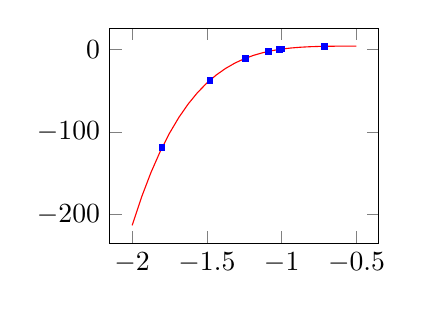
\begin{tikzpicture}
\begin{axis}
\addplot[domain=-2:-0.5, color=red]{8*x^5 + x^4 + 9*x^2 + 7*x + 5};
\addplot[only marks, mark=square*, color=blue, mark size=1pt]
coordinates{(-0.714286, 3.364669)(-1.800553, -119.313308)(-1.479526, -37.579659)(-1.243298, -11.168061)(-1.089281, -2.806756)(-1.016449, -0.429153)(-1.000672, -0.016829)};
\end{axis}
\end{tikzpicture}
\caption{Newton法}
\label{fig:new_poly}
\end{figure}
\par 牛顿法迭代9次后即达到目标精度, 显著优于二分法.
\end{frame}

\begin{frame}
\frametitle{结论}
可以看出, 不管是理论上还是实际例子中, Newton法在求解函数的根问题上都优于二分法, 不过其有可导的前提, 在应用上没有二分法广泛.
\end{frame}

\end{document}